\documentclass[11pt]{article}
\usepackage{amsmath,amssymb,amsthm}
\usepackage{enumitem}
\usepackage{setspace}
\usepackage{xcolor}
\usepackage{graphicx}
\usepackage{geometry}
\usepackage{float}
\usepackage{titlesec}
\usepackage{subfigure}
\usepackage{caption}
\captionsetup{figurewithin=section}
\usepackage{amsmath}
\usepackage{enumitem}
\usepackage{amssymb}

\DeclareMathOperator*{\E}{\mathbb{E}}
\let\Pr\relax
\DeclareMathOperator*{\Pr}{\mathbb{P}}

\newcommand{\eps}{\varepsilon}
\newcommand{\inprod}[1]{\left\langle #1 \right\rangle}
\newcommand{\R}{\mathbb{R}}

\newcommand{\handout}[5]{
  \noindent
  \begin{center}
  \framebox{
    \vbox{
      \hbox to 5.78in { {\bf \centering ECE-GY 9243/ME-GY 7973} \hfill #2 } 
      \vspace{5mm} 
      \hbox to 5.78in { {\bf \Large Optimal and Learning Control for Robotics}}
      \vspace{4mm}
      \hbox to 5.78in { {\Large \hfill #5  \hfill} }
      \vspace{2mm}
      \hbox to 5.78in { {\em #3 \hfill #4} }
    }
  }
  \end{center}
  \vspace*{4mm}
}

\newcommand{\lecture}[4]{\handout{#1}{#2}{#3}{Name: #4}{ #1}}

\newtheorem{theorem}{Theorem}
\newtheorem{corollary}[theorem]{Corollary}
\newtheorem{lemma}[theorem]{Lemma}
\newtheorem{observation}[theorem]{Observation}
\newtheorem{proposition}[theorem]{Proposition}
\newtheorem{definition}[theorem]{Definition}
\newtheorem{claim}[theorem]{Claim}
\newtheorem{fact}[theorem]{Fact}
\newtheorem{assumption}[theorem]{Assumption}

% 1-inch margins, from fullpage.sty by H.Partl, Version 2, Dec. 15, 1988.
\topmargin 0pt
\advance \topmargin by -\headheight
\advance \topmargin by -\headsep
\textheight 8.9in
\oddsidemargin 0pt
\evensidemargin \oddsidemargin
\marginparwidth 0.5in
\textwidth 6.5in

\parindent 0in
\parskip 1.5ex

\begin{document}

\lecture{Homework 1}{Spring 2019}{Prof.\ Ludovic Righetti}{Yunian Pan}

\section{exercise 1 [Convex optimization with linear equalities]}
 The optimization problem is:
\begin{align}
\min_{\textbf{x}} & \ \frac{1}{2} \textbf{x}^{\top}\textbf{Q}\textbf{x} \\ \nonumber
\text{subject to} & \  \textbf{Ax} = \textbf{b}   \nonumber
\end{align} 
 
 The Lagrangian of the optimization problem is:
 \begin{align}
 \mathcal{L} = \frac{1}{2} \textbf{x}^{\top}\textbf{Q}\textbf{x} + \lambda^{\top} (\textbf{Ax} - \textbf{b})
 \end{align}

Use the KKT condition we get: 
\begin{align}
\frac{1}{2}(\textbf{Q}+\textbf{Q}^{\top})\textbf{x} + \textbf{A}^{\top} \lambda &= 0 \\ 
\textbf{Ax} - \textbf{b} &= 0
\end{align}

Solve the KKT system, it's known that $\textbf{Q} \in R^{n\times n} > 0$ $\implies \textbf{Q}$ is invertible, $\textbf{A} \in R^{m \times n} \text{ is full rank}$ $\implies \textbf{A}(\textbf{Q}+\textbf{Q}^{\top})^{-1}\textbf{A}^{\top}$ is invertible, thus:
\begin{align}
\lambda &= - \frac{1}{2} (\textbf{A} (\textbf{Q}+\textbf{Q}^{\top})^{-1} \textbf{A}^{\top})^{-1} \textbf{b} \label{lambda}\\  
\textbf{x} &= (\textbf{Q}+\textbf{Q}^{\top})^{-1}\textbf{A}^{\top} (\textbf{A} (\textbf{Q}+\textbf{Q}^{\top})^{-1} \textbf{A}^{\top})^{-1} \textbf{b} \label{x}
\end{align}

now our problem is:
\begin{equation}
\begin{aligned}
\min_{\textbf{x}} & \ \frac{1}{2} \textbf{x}^{\top} \begin{bmatrix}
10 & 1 & 0\\
1& 100 & 2\\
0 & 2 & 1 \\
\end{bmatrix}
\textbf{x}  \\ 
\text{subject to}  &\ \textbf{1}^{\top}\textbf{x} = 1 
\end{aligned} 
\end{equation} 

where $\textbf{A} = \textbf{1}^{\top} = [1 \  1 \  1]$ and $\textbf{Q} =  \begin{bmatrix}
10 & 1 & 0\\
1& 100 & 2\\
0 & 2 & 1 \\
\end{bmatrix}$, apply formula $\ref{lambda}$ and $\ref{x}$, we get the result $\textbf{x}$:
\begin{equation}
\textbf{x}^{\top} = \left[ \begin{array}{ccc}   0.09090909,\ \ -0.01030928, \ \ 0.91940019  \end{array} \right] \nonumber
\end{equation}

\section{exercise 2 [Netwon’s method]}

\begin{itemize}
\item[$\bullet$] As implemented in jupyter notebook, Newton's method converges much faster than gradient descent.
\item[$\bullet$] As implemented in jupyter notebook, the results are as follows:
\begin{itemize}
\item[$\bullet$] As shown in $\ref{(1)}$, $f(x)\ with\ x\in [-10, 10]$, start from $x_0 = 6.5$ the iteration went all the way down to the convergence extremal point.
\begin{figure}[htbp]
  \centering
  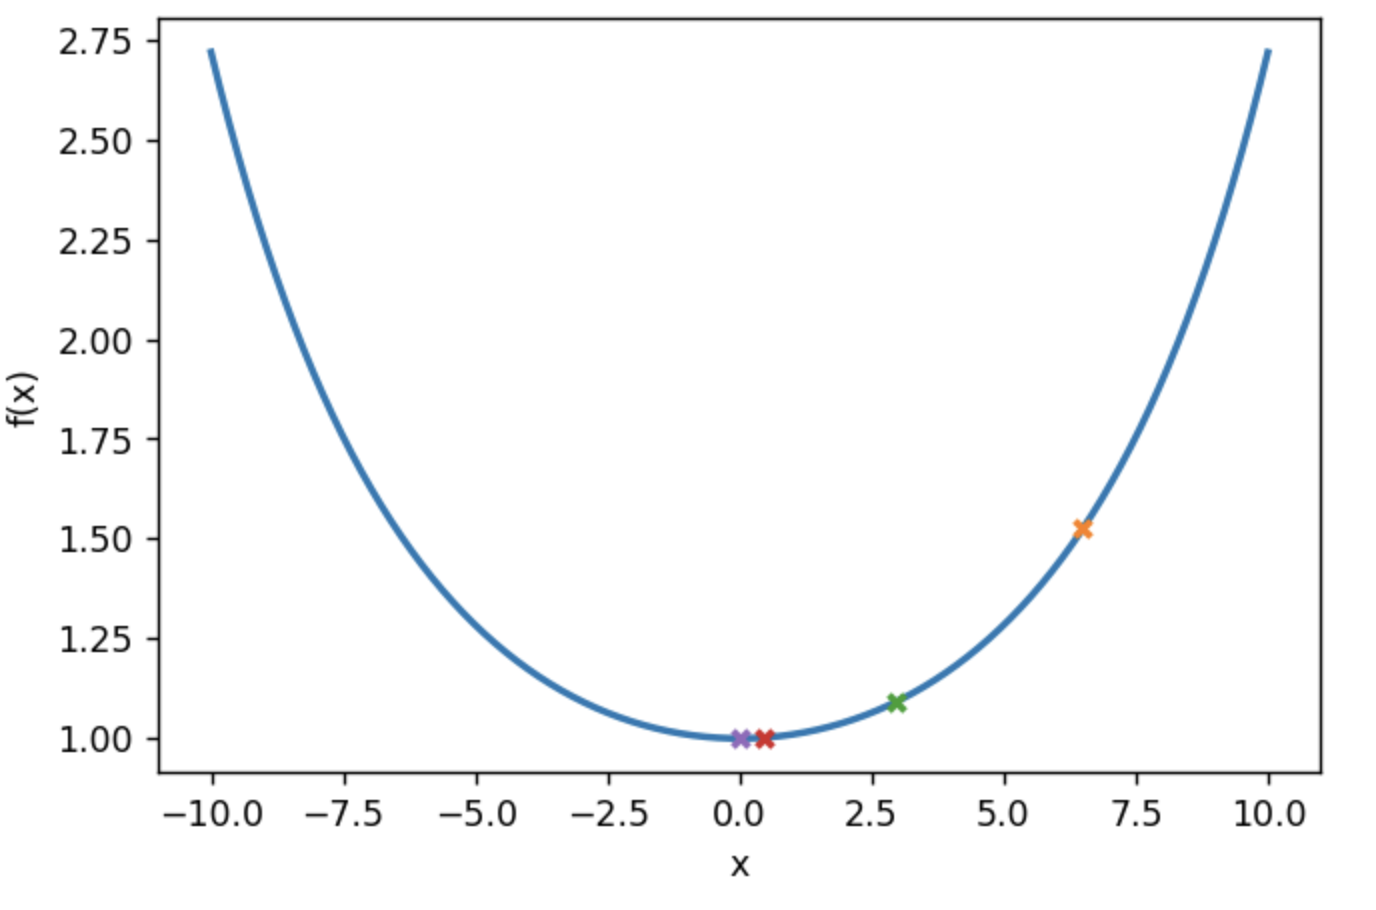
\includegraphics[width = .6\textwidth]{1.png}
  \caption{}
  \label{(1)}
  \end{figure}
\item[$\bullet$] As shown in $\ref{(2)}$, $f(\textbf{x}) \  \textbf{x} \ \text{in the box }\{(x,y)|x \in [-10,10], y\in [-10,10]\} $, the converging process goes in almost one direction.
\begin{figure}[htbp]
\centering
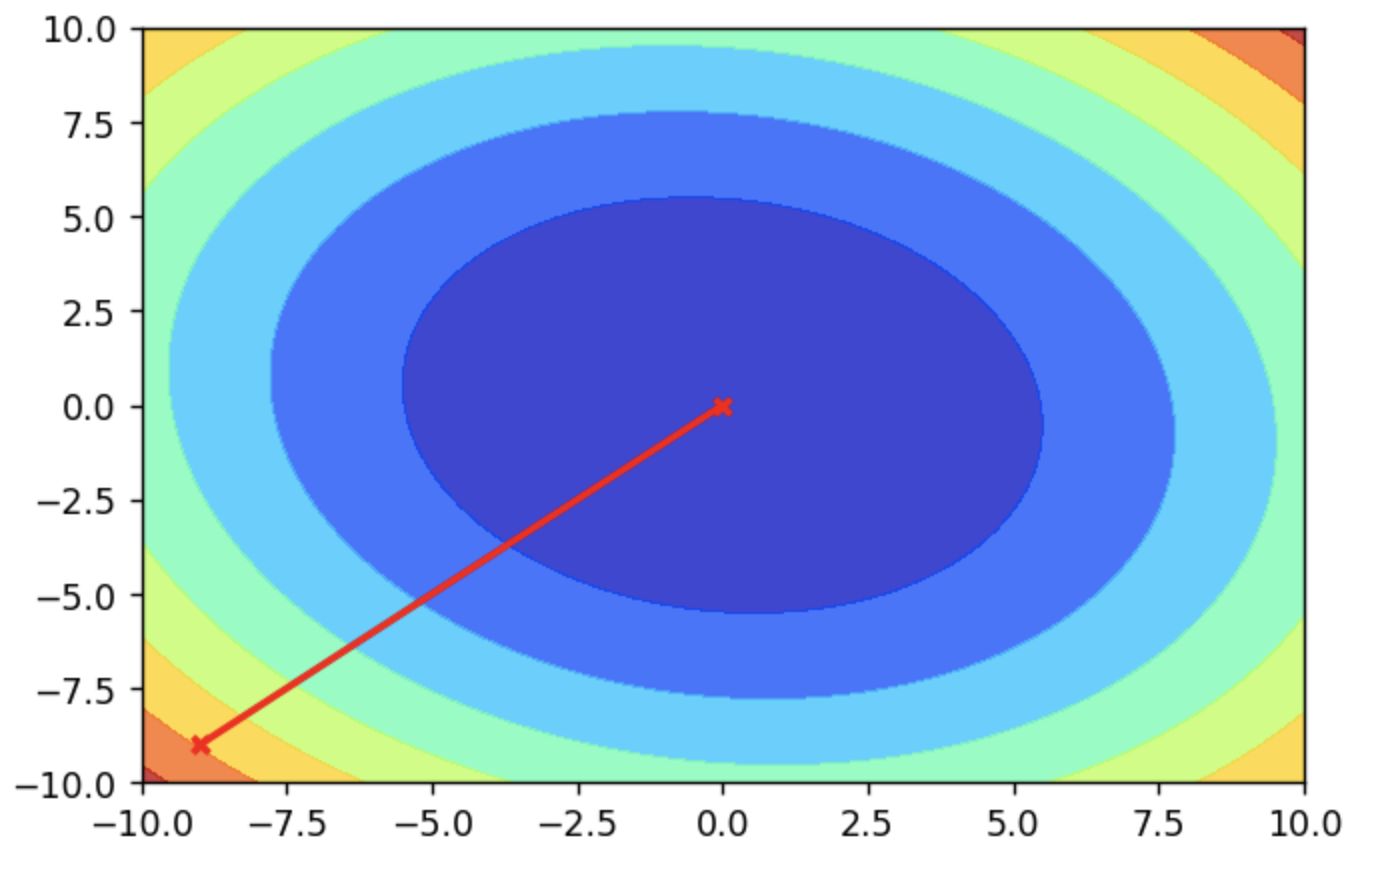
\includegraphics[width = .6\textwidth]{2.png}
\caption{}
\label{(2)}
\end{figure}
\end{itemize}
\item[$\bullet$] comparison shown in $\ref{(3)}$ and $\ref{(4)}$, since the points of convergence can be easily computed that $x_c = 0 \text{ and }\textbf{x}_c = (0, 0)$, I compared the converging process with these extremal points instead of the final results, as there's a tolerance below which the iteration stops, the true error will never goes to 0.

\begin{figure}[htbp]
\centering
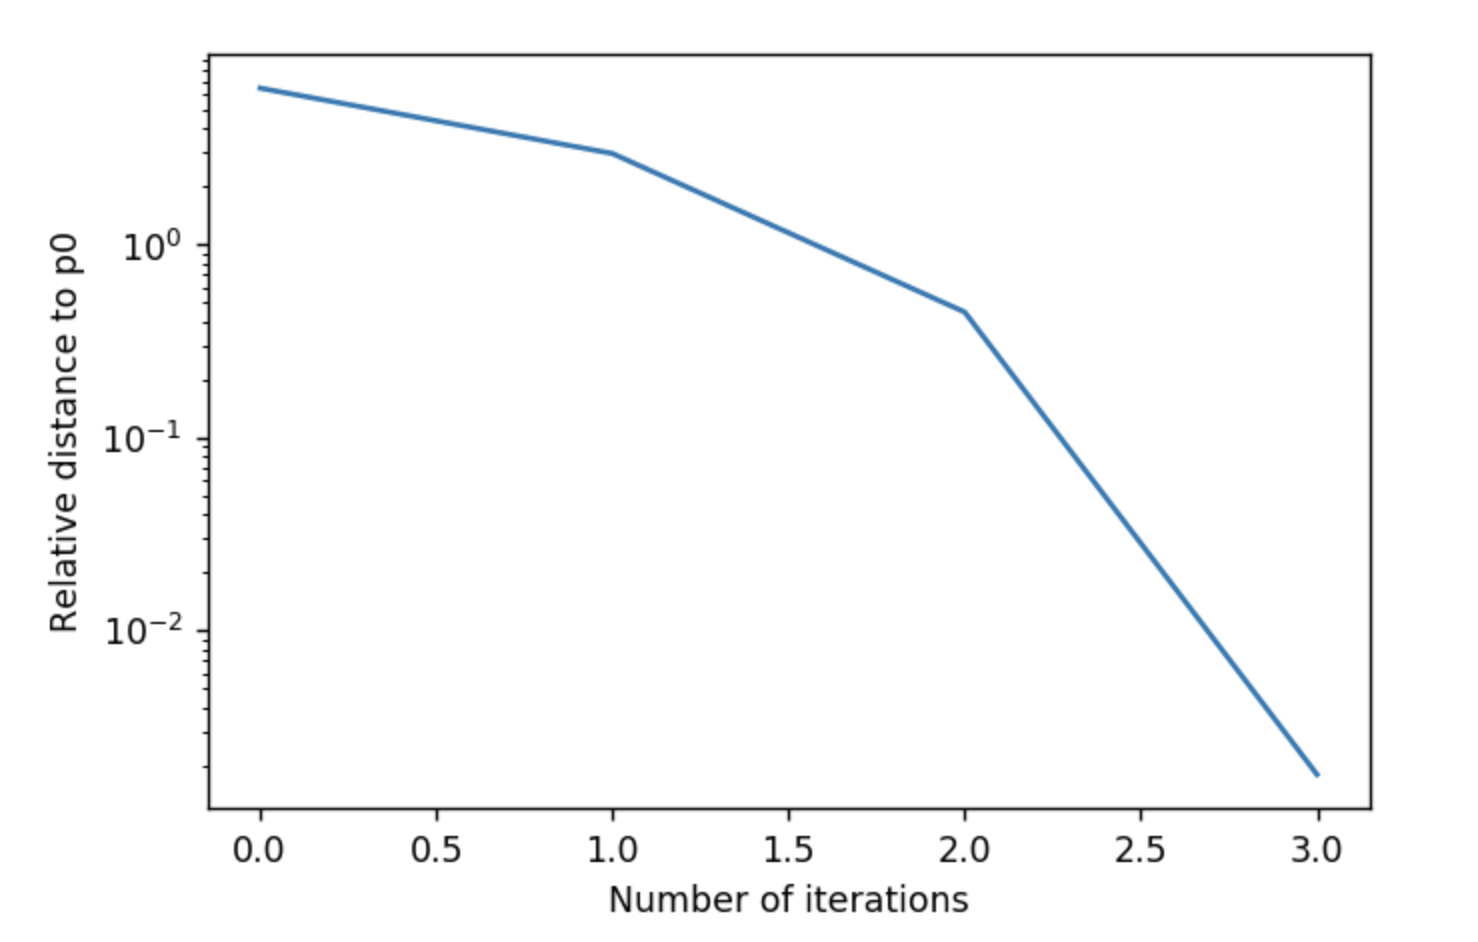
\includegraphics[width = .67\textwidth]{3.png}
\caption{$f(x) = e^{\frac{x^2}{100}}$}
\label{(3)}
\end{figure}
\begin{figure}[htbp]
\centering
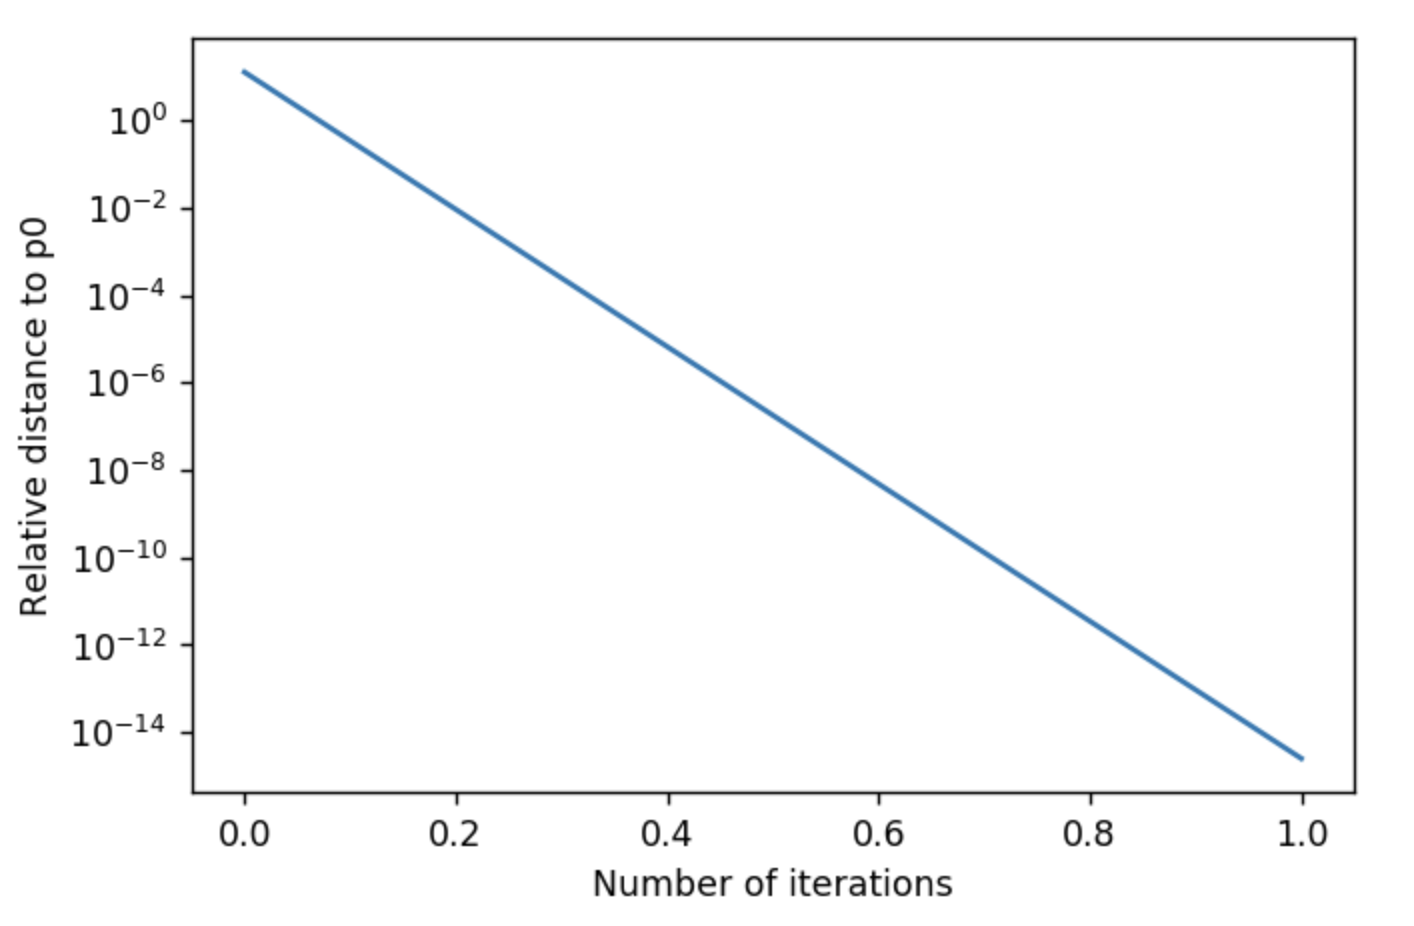
\includegraphics[width = .67\textwidth]{4.png}
\caption{$f(x) = x^{\top}Q x$}
\label{(4)}
\end{figure}

Note that as tolerance goes down to $10^{-10}$ or even smaller, the number of iteration increases to some degree.
\end{itemize}


\section{exercise 3 [Linear Least Squares]}
\begin{itemize}
\item[$\bullet$] As implemented in jupyter notebook, I modified the function so that it can process cross-validation to find the best polynomial order without overfitting.
\begin{itemize}
\item[$-$]  The order of polynomial that best fits the data is uncertain because the split of training and testing set is random, it usually takes on a value between 3 and 6 as I tried from 1 to 10, $\ref{(5)}$ shows an example of best order.
\begin{figure}[htbp]
\centering
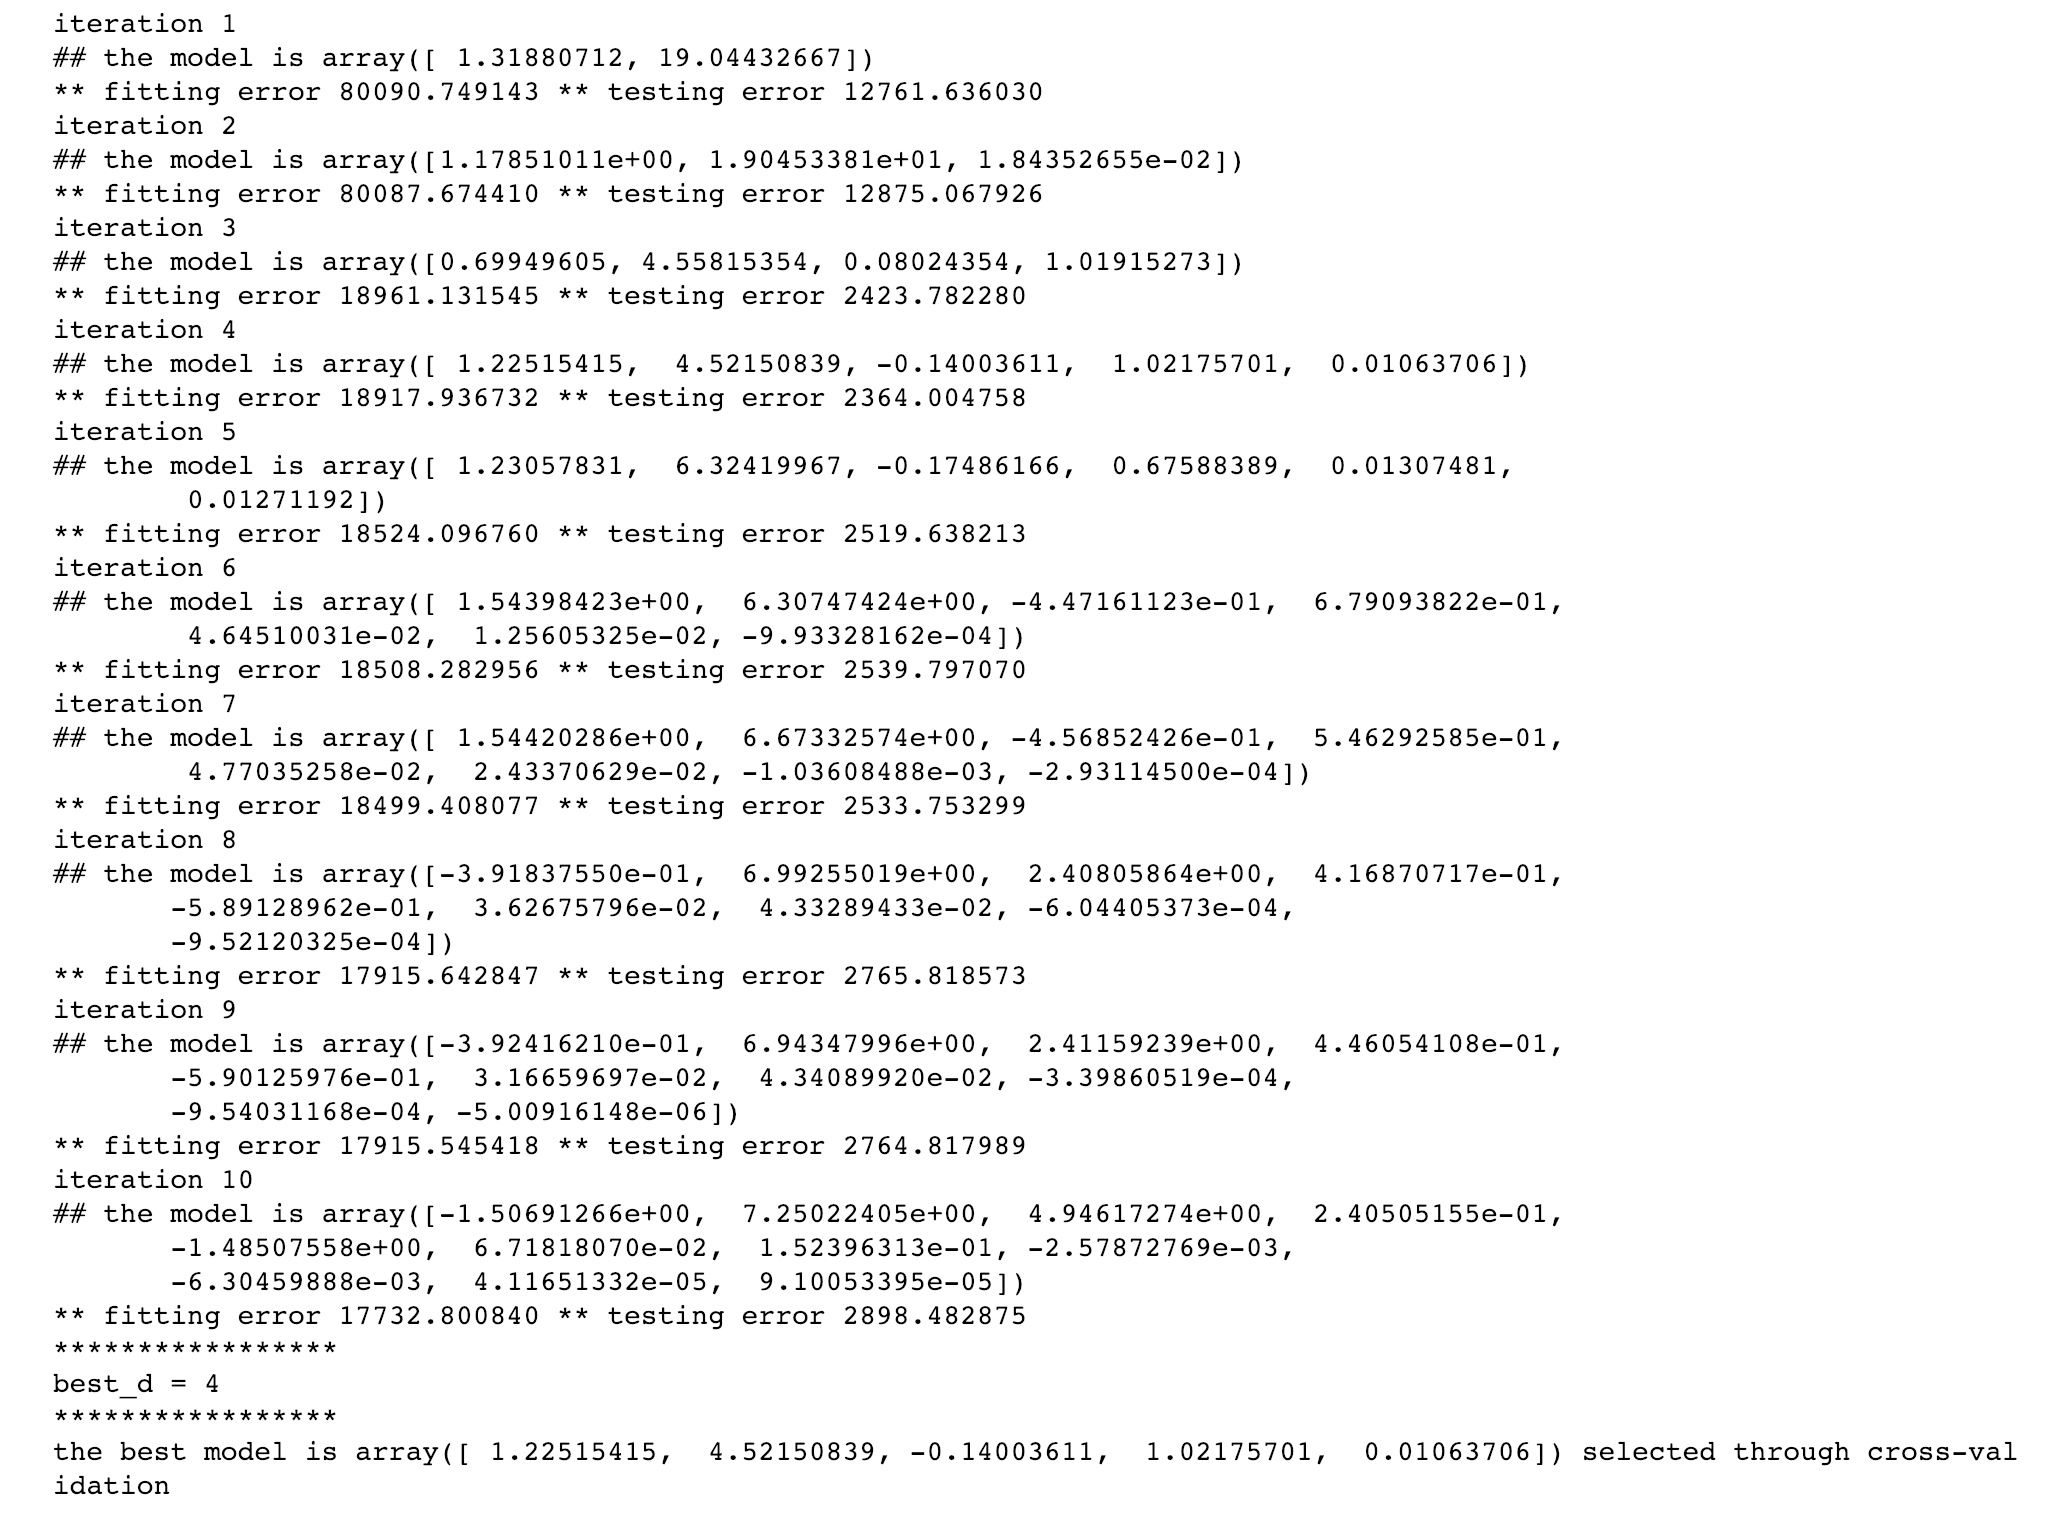
\includegraphics[width = 1.1\textwidth]{5.png}
\caption{}
\label{(5)}
\end{figure}
 
 The best order is 4 in this case because the model with $degree = 4$ has the lowest testing error, which means it predicts the data more reasonably while fits the dataset well.
 
 \item[$-$] The polynomial coefficients are in the selected model, which is [1.22515415,  4.52150839, -0.14003611,  1.02175701,  0.01063706].
 
 \item[$-$] Plot the overlaid function as shown in $\ref{(6)}$. The fit looks good, despite the fact that some of the data points are out of the curve, those data points can be viewed as noise.
 \begin{figure}[htbp]
\centering
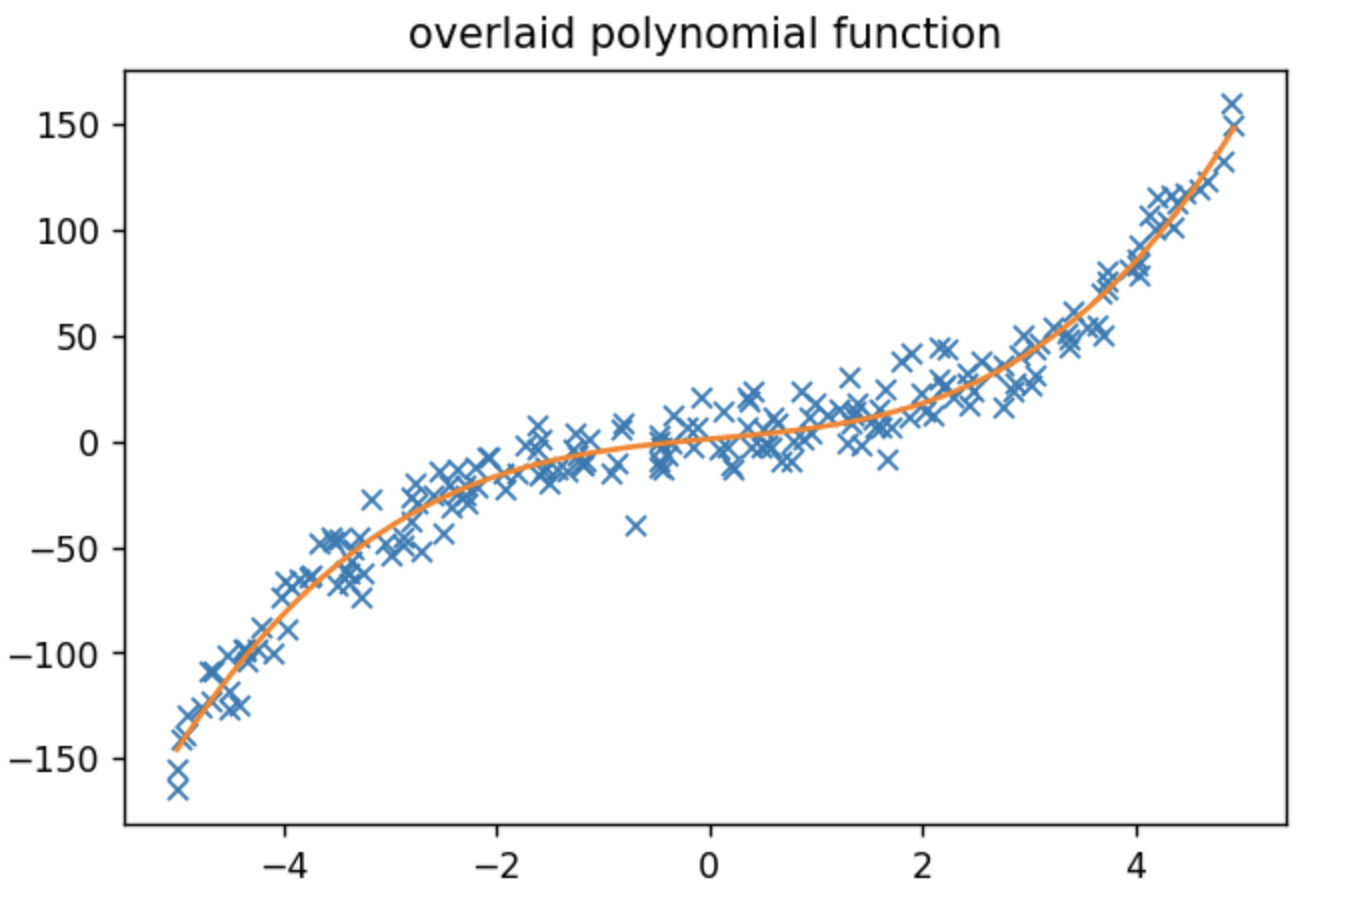
\includegraphics[width = .75\textwidth]{6.png}
\caption{}
\label{(6)}
\end{figure}
\end{itemize}
\end{itemize}
\begin{itemize}
\item[$\bullet$]Since it is in fact possible to use functions to mapp the data as long as the mapping is of the form $y = \sum_{k} a_k f_k(x)$ where $f_k$ is an arbitrary function. Now that we want to fit periodic functions of the form:
\begin{equation}
 y_n  = a_0 + \sum_{k=1}^{K}a_k \cos(kT2\pi x_n) + \sum_{k=1}^{K}b_k \sin(kT2\pi x_n) \nonumber
\end{equation}
\begin{itemize}
\item[$-$] The optimization problem can be written as:
\begin{equation}
\begin{aligned}
\min & \  || y - \hat{y}||^2 \\ \nonumber
\text{subject to} & \ \hat{y} = F(\textbf{x})\textbf{w} \\ 
\end{aligned}
\end{equation}
\begin{equation}
\begin{aligned}
\text{where }  F(\textbf{x})& =  \left[\begin{matrix}
1  &  \cos(2\pi T x_1)  & \cdots\ &\cos(2\pi KT x_1) &\sin(2\pi T x_1)& \cdots &\sin(2\pi KT x_1)\\
1  &  \cos(2\pi T x_2)  & \cdots\ & \cos(2\pi KT x_2)  &\sin(2\pi T x_2)&\cdots &\sin(2\pi KT x_2)\\ 
\vdots   & \vdots & \ddots  & \vdots  & \vdots & \ddots & \vdots \\
1 &  \cos(2\pi T x_n)  & \cdots\  & cos(2\pi KT x_n) &\sin(2\pi T x_n)& \cdots &\sin(2\pi KT x_n)\\
\end{matrix} \right]\nonumber \\
\textbf{w}^{\top} &= \left[a_0 \  a_1 \ldots a_K \  b_1 \ \ldots b_K\right]  \nonumber 
\end{aligned}
\end{equation}
\item[$-$] As implemented in jupyter notebook. We take derivative to obtain the parameters:
\begin{equation}
\begin{aligned}
\mathcal{L} &= ||y - \hat{y} ||^2 \nonumber \\
\cfrac{\partial \mathcal{L}}{\partial {\textbf{w}}} &= \cfrac{\partial }{\partial {\textbf{w}}} (\textbf{y} - F(\textbf{x}) \textbf{w})^{\top}(\textbf{y} - F(\textbf{x}) \textbf{w})\nonumber \\
& = -2F(\textbf{x})^{\top} \textbf{y} + 2 F(\textbf{x})^{\top}F(\textbf{x})\textbf{w} \nonumber \\
\end{aligned}
\end{equation}
Let $\cfrac{\partial \mathcal{L}}{\partial {\textbf{w}}} = 0 \implies \textbf{w} = (F(\textbf{x})^{\top}F(\textbf{x}))^{-1}F(\textbf{x})^{\top} \textbf{y}$, which is quite similar to the polynomial solution.
\item[$-$] Assuming $T=1$, start from $K = 2$, the testing error and training error already decrease to 0, as shown in $\ref{(7)}$.
 \begin{figure}[htbp]
\centering
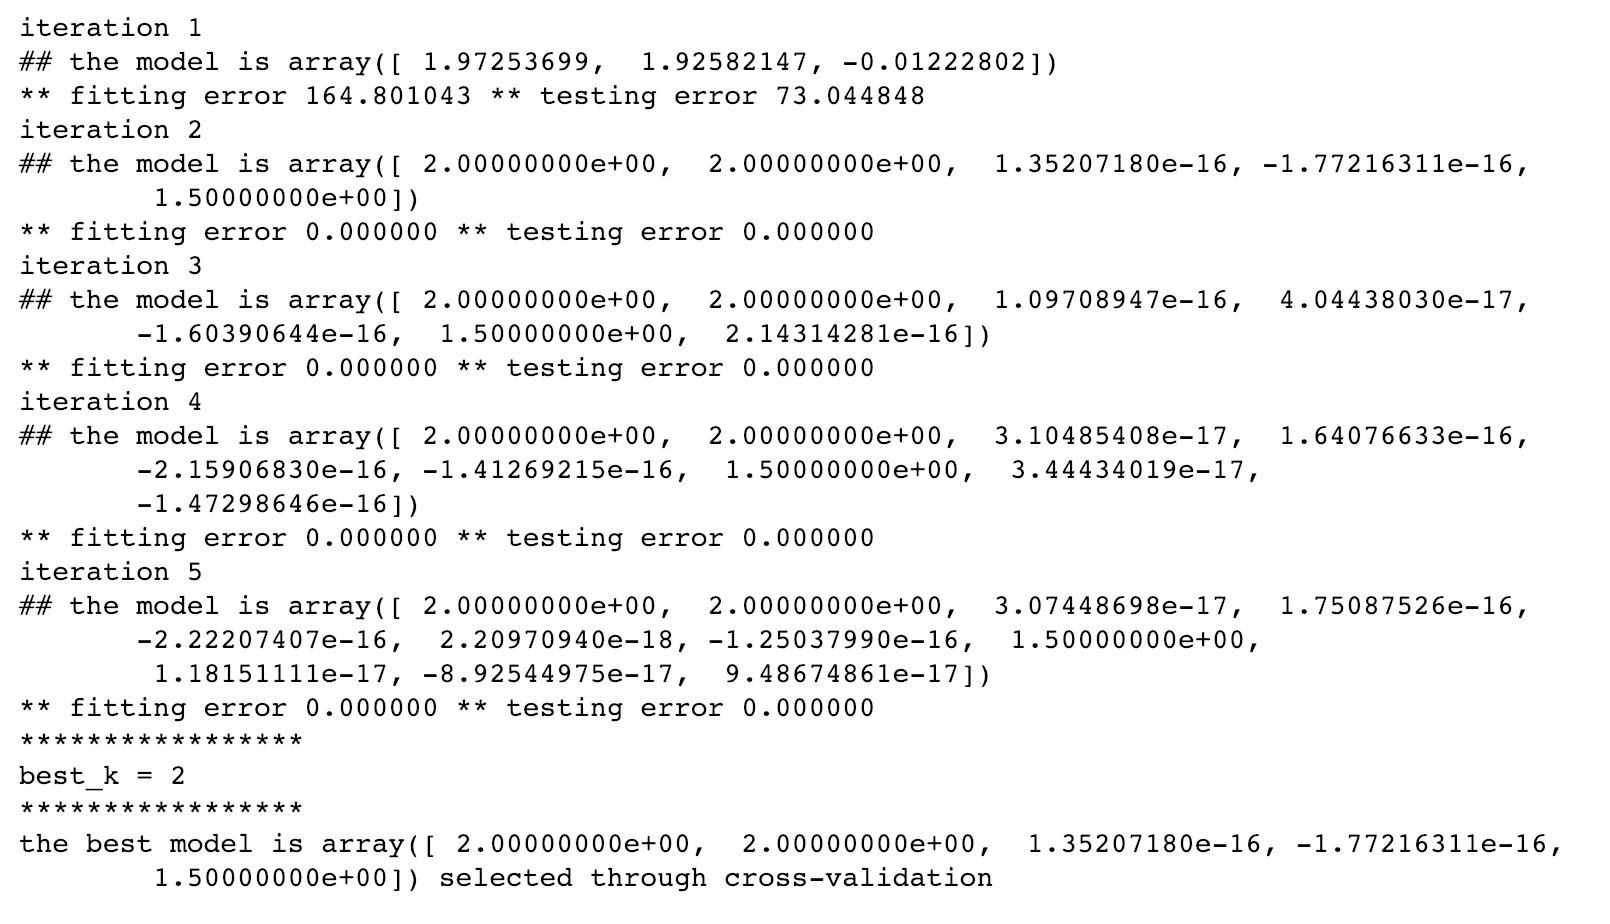
\includegraphics[width = .85\textwidth]{7.png}
\caption{}
\label{(7)}
\end{figure}
\item[$-$] $\ref{(8)}$ gives the overlaid function, which looks good.
\begin{figure}[htbp]
\centering
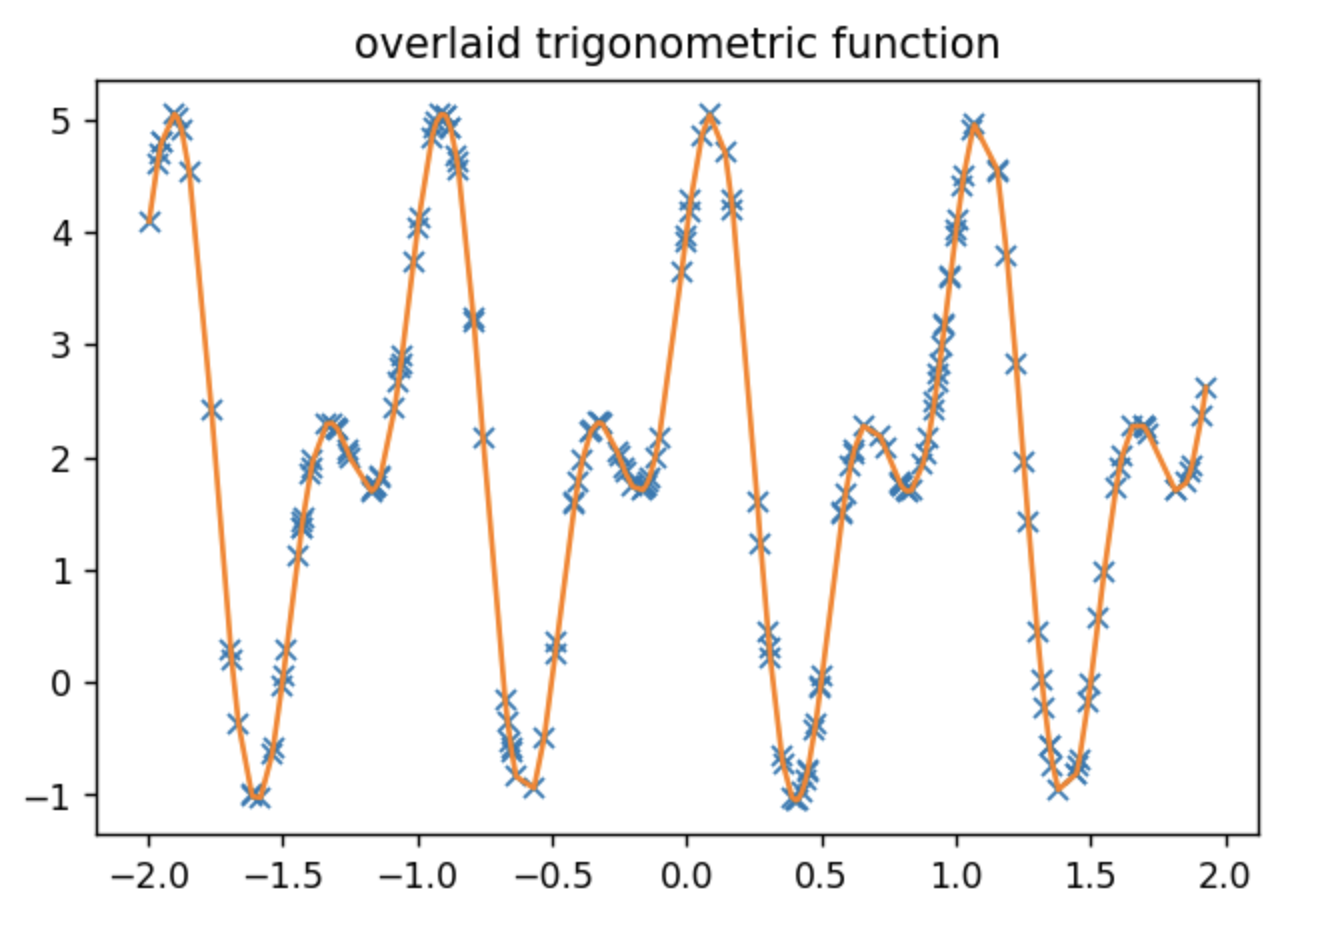
\includegraphics[width = .6\textwidth]{8.png}
\caption{}
\label{(8)}
\end{figure}
\end{itemize}
\end{itemize}

\end{document}
